\section*{Motivation}\label{sec:intro}
\addcontentsline{toc}{section}{Motivation}
The goal of this assignment is to get some hands-on experience in formulating a dynamic optimization problem, discretizing and realize the problem on a computer, and finally solving it. Another goal of the assignment is to teach us some ways to implement omptimal control with and without feedback in a modern environment using Simulink and MATLAB. All of this is realized on a helicopter at one of the labs at NTNU.

This project is part of the mandatory coursework in the course TTK4135, Optimization and Control, at NTNU in the spring of 2018.

The physical setup for this project consists of a two-rotor helicopter fixed on an arm with a counterweight on the other end. This is again connected to another arm which is connected to the base. Figure \cref{fig:heli} shows a force representation of our helicopter setup. The different angles are measured with optical position sensors. The helicopter is then connected to a QuaRC-server that we use our workstation and simulink to interface with.


\begin{figure}[tp]
	\centering
	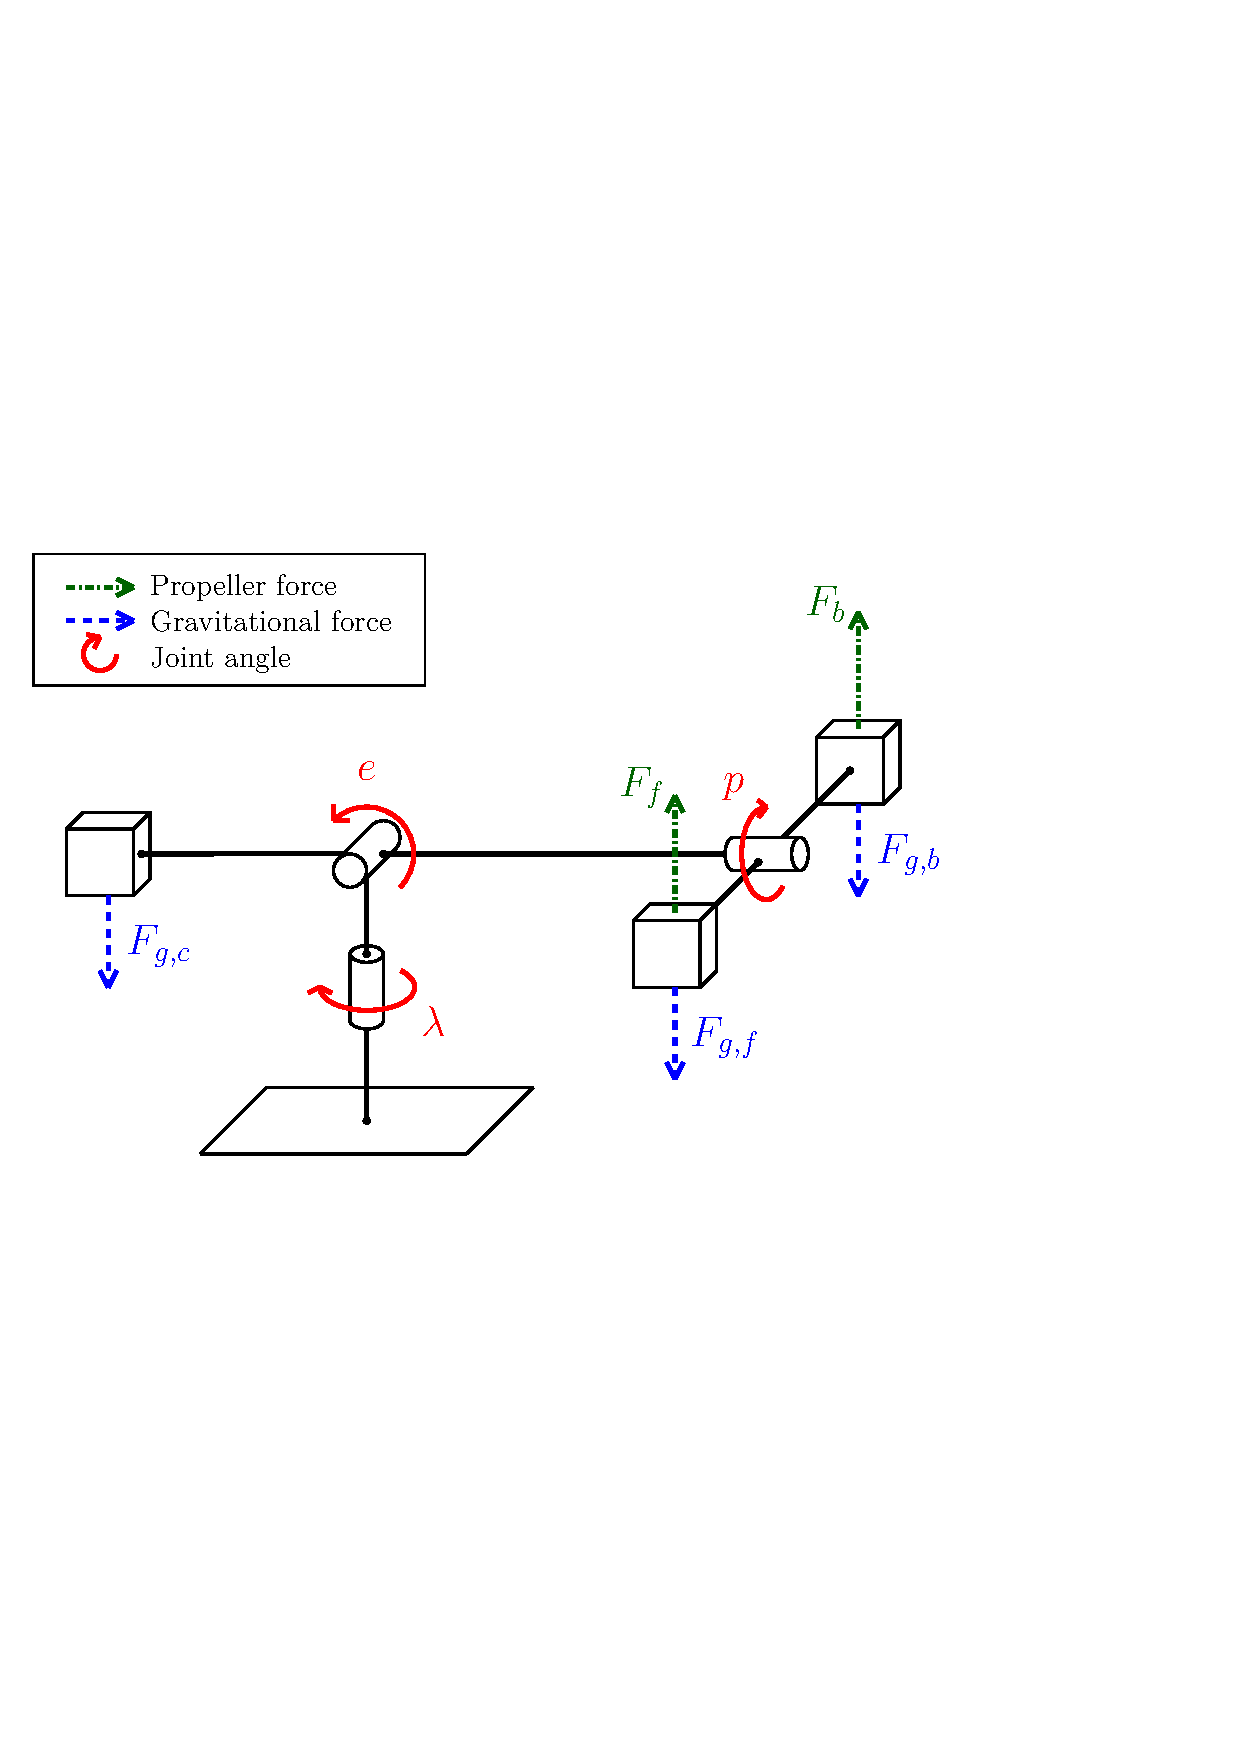
\includegraphics[width=1.00\textwidth]{figures/forces.pdf}
	\caption{Force diagram representation of our helicopter.}
\label{fig:heli}
\end{figure}